\chapter{Introducción}

\section{Descripción General}
% Desde los principios de la tecnología de semiconductores, los sistemas electrónicos han venido experimentando un constante crecimiento en
% complejidad, debido a que las prestaciones que tiene que ofrecer una aplicación concreta son cada vez mayores y de naturalezas más diversas. Esto ha
% dado lugar a que un sistema tenga a la vez restricciones aparentemente incompatibles, como pueden ser de trabajo en tiempo real, de tolerancia a
% fallos o de procesado de grandes flujos de datos. Este incremento de complejidad y diversidad en las restricciones ha motivado la aparición de diseños
% híbridos en los que interactúan elementos hardware y software, ya que dichos elementos pueden complementarse para resolver problemas de distinta
% naturaleza. 
% 
% El codiseño hardware/software es la tarea de diseñar el sistema hardware y generar el código del sistema software de manera conjunta (sistema mixto),
% de tal forma que el comportamiento del sistema global tenga las mismas prestaciones que en la descripción funcional y cumpla con objetivos que
% serían inalcanzables mediante metodologías tradicionales de diseño. Esto motivó al desarrollo de una solución que involucra Intelectual Property
% Cores (IP-Cores) que interactuen con aplicaciones de usuario por medio de un procesador estándar a través de un driver corriendo en un Sistema
% Operativo.
% 
% Entre las alternativas para diseñar e implementar un hardware específico encontramos ASICs  (Application-specific integrated circuit), FPGAs
% (Field-programmable gate array), CPLDs (Complex Programmable Logic Device) entre otros. El uso de ASICs posibilita desarrollos con producción a gran
% escala a bajo costo y es de masiva utilización en este tipo de aplicaciones. Los  CPLD  y las FPGA son circuitos de de alta densidad programables por
% el usuario en un tiempo reducido y sin la necesidad de verificación de sus componentes, tarea ya realizada por el fabricante al tratarse de un
% producto estándar. El procesamiento digital de señales , prototipado de ASICs , tratamiento de imágenes , reconocimiento de voz , glue logic son
% algunas de las aplicaciones de este tipo de dispositivos. Existen diferentes formas de llevar adelante el diseño e implementación de un sistema
% digital para FPGA, entre ellas tenemos la realización de un diseño esquemático , herramientas específicas (provistas por el fabricante) y la
% utilización de un lenguaje de descripción de hardware HDL (Hardware description language) entre los que  se encuentran lenguajes como Verilog y VHDL,
% ambos de gran aceptación en los ambientes industrial y académico. Estos lenguajes proporcionan gran versatilidad para el desarrollo de hardware,
% permitiendo especificar, diseñar, simular y verificar sistemas digitales complejos, mediante el apoyo de un universo de herramientas EDA (Electronic
% Design Automation).
% Actualmente las FPGA cuentan con una gran cantidad de recursos disponibles (Compuertas lógicas , Bloques de RAM) para implementar diseños digitales
% complejos. Las FPGA pueden ser usadas para implementar cualquier función lógica que un ASIC  pueda realizar. Una de las grandes ventajas del uso de
% FPGA en la etapa de prototipado es su capacidad de reconfigurar el diseño parcial o totalmente para su actualización o corrección de errores con un
% costo relativamente bajo a diferencia del prototipado sobre ASICs. Durante la etapa de producción los  ASIC resultan de muy bajo costo respecto de la
% producción de FPGA y esto se traduce en una gran ventaja para desarrollos que deben ser producidos a gran escala.
% Las arquitecturas reconfigurables combinan parte de la flexibilidad del software con la gran performace del hardware utilizando chips reconfigurables
% como FPGAs. Una opción de gran potencialidad son las arquitecturas reconfigurables run-time o dinámicas que se sostienen en DRL (Dynamically
% reconfigurable logic ). Un ejemplo de esto es la familia Virtex de Xilinx, que es parcialmente reconfigurable en tiempo de ejecución, este método se
% conoce como run-time. Claramente este tipo de dispositivos puede ser usado como arquitecturas destino de codiseños hardware/software (HW/SW) que
% proveen la flexibilidad de los procesadores software y la eficiencia y rendimiento de los coprocesadores hardware.
% El desarrollo de aplicaciones de software se ve limitado a los recursos disponibles en los microprocesadores comerciales. El software necesita del
% soporte de un procesador para su ejecución, así la elección de este elemento conlleva algunas dependencias respecto de las herramientas a utilizar ,
% algunas de estas son : compiladores , ensambladores , depuradores y herramientas de simulación. Con ellas se logra trasladar el software a un entorno
% de ejecución adecuado dentro del procesador y depurarlo . El lenguaje de programación elegido debe permitir trabajar con el nivel de abstracción
% necesario para simplificar la tarea de desarrollo de software. El lenguaje ‘C’ es uno de los más utilizados para desarrollar aplicaciones que
% requieran ,por ejemplo , de compilación cruzada (Cross-compilling) y se complementa con las herramientas libres de compilación y depuración como son
% GCC y GDB.
% Los nuevos proyectos a veces requieren nuevas características de los cores existentes. El proveedor del núcleo puede hacer estas modificaciones
% (solución comercial) con un incremento sustancial del coste del núcleo. Otra posibilidad (Solución Ad-hoc) es el uso de cores de código abierto con
% el fin de crear un núcleo de desarrollo adaptable. El enfoque de código abierto tiene  varias ventajas: el núcleo posee un costo muy bajo e inclusive
% cero, los usuarios puede tener acceso al código fuente y hay un grupo de desarrolladores que proporcionan conocimientos para mantener y mejorar el
% núcleo. Sin embargo, también puede tener varias desventajas como la inestabilidad (el grupo de cambio o de desarrollo desaparece), desarrollo
% incompleto, deficiente , documentación pobre y una mala metodología de verificación.Los microprocesadores “softcore”(núcleo software) son aquellos
% cuyo hardware está íntegramente implementado en un lenguaje de descripción de hardware.Posibilitan un desarrollo confiable con facilidad de ajustar
% el mismo a las necesidades de aplicación que deben satisfacerse e incluso el desarrollo de microprocesadores doble o múltiple núcleo. Entre los
% microprocesadores softcore de código privativo más importantes encontramos MicroBlaze de Xilinx , Nios y Nios II de Altera y Cortex M1 de ARM. Como
% contrapartida encontramos los microprocesadores softcore  Open Source (Código Abierto)  OpenSPARC T1 de Sun (64 bits) y OpenRISC de Open Cores.
% 
% 
% El procesador OpenRISC de 32 bits se comunica con sus periféricos por medio de un bus tipo Wishbone , también de código abierto.  OpenRISC puede ser
% implementado fácilmente en chips de cualquier fabricante (Xilinx , Altera , Actel) razón por la cual es el elemento central de algunos proyectos SoC
% de código abierto tales como MinSoC de OpenCores  u  ORPSoC de OpenCores.
% Los sistemas embebidos SoC (System on a chip) integran los componentes de hardware necesarios para cumplir una funcionalidad específica. Una
% arquitectura típica SoC integra un procesador , un procesador o un núcleo DSP como elemento central , bloques de memoria (ROM , RAM , EEPROM) ,
% periféricos , osciladores , entre otros.

\section{Objetivos}
\subsection{Objetivo General}

Implementar un System on Chip OpenSource con Microprocesador Softcore embebido que soporte un Sistema Operativo libre, con la finalidad de entregar
un sistema integral FPGA-SoC-Sistema Operativo completamente funcional y bajo licencia GPL v2. %o LGPL

\subsection{Objetivo Específico}
\begin{itemize}
\item Seleccionar, analizar y determinar la factibilidad de implementación de un microprocesador Softcore en FPGA.
% No es seleccionar el SoC tamb 
\item Establecer un System on Chip Open Source donde poder implementar un Softcore.
%o LGPL ???
\item Determinar los Sistemas Operativos con licencia GPL v2 que poseean las prestaciones funcionales adecuadas para su utilización en Sistemas
Embebidos de propósito específico(Por ej.: Sistemas de tiempo real).
\end{itemize}

\section{Motivación} 

Existe un grupo de cores Softcore de código abierto que no están limitados por la tecnología. Los cores destacados de microprocesadores de 32 bits,
son los procesadores SPARC LEON OpenRISC 1200 , y el core de LatticeMico32. Usar cores de código abierto va unido a una serie de conceptos como:
\begin {itemize}
\item
\textit{Flexibilidad}  Si el código fuente está disponible, los desarrolladores pueden modificar el código de acuerdo a sus necesidades. Además, se
produce un flujo constante de ideas que mejoran la calidad del código.
\item 
\textit{Fiabilidad y seguridad}  Con muchos programadores a la vez escrutando el mismo trabajo, los errores se detectan y corrigen antes, por lo que
el producto resultante es mas fiable y eficaz que el comercial.
\item 
\textit{Rapidez de desarrollo}  Las actualizaciones y ajustes se realizan a través de una comunicación constante vía Internet.
\item 
\textit{Relación con el usuario} El programador se acerca mucho mas a las necesidades reales de su cliente, y puede crear un producto específico para
él.
 \end {itemize}
 
Obtener un Sistema Integral de código abierto en donde se tiene código HDL, assembler y C disponible para adaptarse de acuerdo a los requerimientos
del proyecto, además de la capacidad de migrar de una plataforma a otra logrando menor dependencia entre el código fuente y la plataforma
objetivo. La portabilidad del código abierto nos permite implementarlo sobre un ASICs (Application-specific integrated circuit) o con modificaciones
menores en cualquier FPGA (Field Programmable Gate Array) de Xilinx, Altera, Lattice, etc. Estos tres de los más grandes proveedores de FPGA  %,% Xilinx , Altera y Lattice ,
ofrecen sus propios microcore RISC de 32bits como lo son Nios de  Altera y Microblaze de Xilinx  Son micro cores en donde el código fuente RTL no se
encuera disponible y solo pueden ser implementados en las FPGA del propio fabricante.

Una de principales ventajas de usar plataformas con FPGA, es que son flexibles y pueden adaptarse a diferentes funciones. Los componentes de
hardware ofrecen mucho mayor rendimiento que el software equivalente. Los cuellos de botella de procesamiento del sistema pueden identificarse y
sustituirse por hardware, de manera que se evita la costosa optimización del software.

\section{Importancia del Problema}

En el diseño del sistema embebido se usan diferentes procesos dependiendo del tipo de sistema, el hardware disponible y la organización que
desarrolle el sistema. Una de las actividades principales en un proceso de diseño de software es la elección del hardware y del sistema operativo que
se efectúa antes del desarrollo del software. Ante tal situación, se debe diseñar el software considerando las restricciones impuestas por las
capacidades del hardware.
Los efectos que influyen dichas elecciones comprenden restricciones de temporización sobre el sistema, limitación en la energía disponible,
experiencia del equipo de desarrollo y límites en el costos del sistema entregable.
 
Se está explorando una línea donde se busca dar al diseñador del sistema embebido una solución flexible en la primera etapa de la elección de
plataforma. Donde a través del análisis de diferentes plataformas de desarrollo OpenSource y privativas se pueda elegir la mejor opción para el tipo
de sistema a desarrollar y los requerimientos de procesamiento.
 
Una vez que se ha elegido la plataforma de ejecución para el sistema, se ha diseñado una arquitectura de proceso y se ha determinado una política de
planeación, es necesario comprobar que el sistema cumplirá sus con sus requerimientos.

\section{Modelo de Desarrollo}

El modelo de desarrollo a utilizar es el Modelo en Espiral tipificado por Ian Sommerville\cite{Etiqueta00}% . El modelo en espiral de ingeniería de software,mostrado en la figura 1.1
, fue originalmente propuesto por Boehm en año 1988, en su artículo "A Spiral Model of Software Development and Enhancement". Propuso un
marco del proceso de software dirigido por el riesgo. Aquí, el proceso de software se representa como una es espiral, cada ciclo en la espiral
representa una fase del proceso de software. Por ende, el ciclo más interno puede relacionarse con la factibilidad del sistema, el siguiente ciclo
con la definición de requerimientos, el siguiente ciclo al diseño del sistema, y así sucesivamente. %Aclarar que lo implementamos para implementar
% HW...

\begin{figure}[h!]
 \begin{center}
  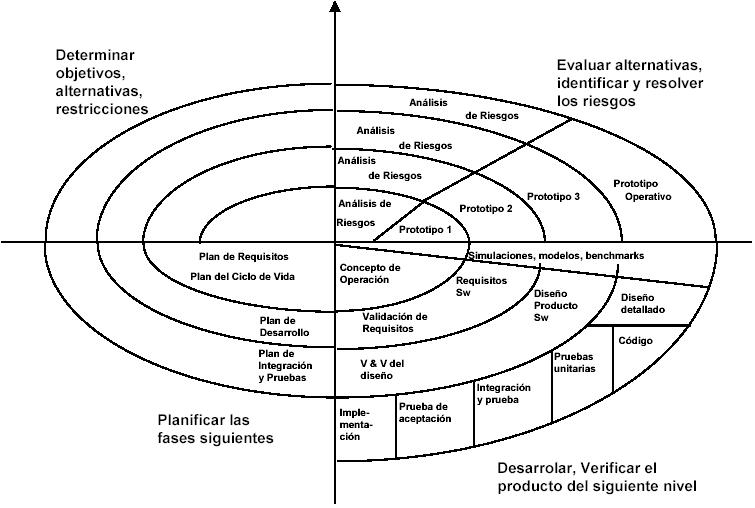
\includegraphics[width=0.5\textwidth,keepaspectratio=true]{./images/ESPIRAL}
  \caption{Etapas del modelo de desarrollo en espiral}
  \label{fig:esquema}
 \end{center}
\end{figure}

Cada ciclo del espiral se divide en 4 sectores:
 
\begin {itemize}
\item 
\textit{Establecimiento de objetivo}  Se definen objetivos específicos para dicha fase del proyecto. Se identifican restricciones en el proceso y el
producto y se traza un plan detallado de gestión. Se identifican los riesgos del proyecto. Dependiendo de estos riegos, se planean estrategias
alternativas que permitan utilizar otros caminos hacia la solución ante sobre la aparición de problemas asociados a estos riesgos.
\item 
\textit{Validación y reducción del riesgo}  En cada uno de los riesgos identificados del proyecto, se realiza un análisis minucioso proponiendo
acciones para reducir dichos riesgos.
\item 
\textit{Desarrollo y validación}  Después de una evaluacion de riesgos, se elige un modelo de desarrollo para el sistema.
\item 
\textit{Planeamiento}  El proyecto se revisa y se toma una decisión sobre si hay que continuar con otro ciclo de la espiral. Si se opta por continuar,
se trazan los planes para la siguente fase del proyecto.
\end {itemize}

Como característica principal de esta metodología es que posee una consideración explícita del riesgo. Informalmente, el riesgo significa
sencillamente que algo puede ir mal. Los riegos originan problemas en el proyecto, como los de confección de agendas y excesos en los costos, por lo
tanto, la disminución de riegos es una actividad sumamente importante en la gestión del proyecto. Un ciclo en la espiral comienza con la elaboración
de objetivos, como el rendimiento y la funcionalidad. Entonces se enumeran formas alternativas de alcanzar estos objetivos y las restricciones
impuestas en cada una de ellas. Cada alternativa se evalúa contra cada objetivo y se identifican las fuentes de riegos del proyecto. El siguiente
paso es resolver estos riesgos mediante actividades de recopilación de información como la de detallar más el análisis, la construcción de prototipos
y la simulación. Una vez que se han evaluado los riesgos se llevará a cabo cierto desarrollo, seguido de una actividad de planificación para la
siguiente fase del proceso.

%El softcore OpenRisc  que se encuentra en el SoC OrpSoc y MinSoc se tiene que implementado en una FPGA  Spartan 3A de Xilinx. Tenemos como fin montar un Linux para validar y verificar el sistema global entregando un sistema funcional bajo licencia libre.
%Actualmente las FPGAs nos birndan la posibilidad de implementar estos proyectos, donde el Hardware y el Software son una misma entidad. Este nuevo enfoque nos permite aprovechar la facilidad de implementar soluciones por Hardware.

\section{Alcance de Estudio}
%En cada etapa ????
Debido al plazo estipulado para el desarrollo del proyecto, el mismo involucra tres etapas: 

\begin {itemize}
\item Especificación y Análisis de requerimientos.
\item Implementación.
\item Testing.
\end {itemize}


\section{Metodología}
%% Primera vez en la facultad???
Considerando que el objetivo planteado es un desarrollo que se realiza por primera vez, se aplicará un desarrollo experimental y de simulación. La
falta de documentación al respecto y al ser un desarrollo de vanguardia son factores que acentúan en esta decisión. Sumado a lo dicho anteriormente,
en el laboratorio donde se desarrolla este proyecto no existen antecedentes de trabajos similares que involucren Microprocesadores Softcore.


%% Esto esta incompleto. 
Se utilizó como metodología en esta implementación el modelo de componentes que define estándares para tal fin, documentación y el
despliegue de componentes.





%%%%% poner en negrita asi \textit{Python} 


